\documentclass[11pt]{article}

\usepackage[margin=1in]{geometry}
\usepackage{graphicx}
\usepackage{subcaption}
\usepackage{booktabs}
\usepackage{amsmath}
\usepackage{siunitx}
\usepackage{tikz}
\usepackage{hyperref}
\usepackage[numbers]{natbib}
\usepackage{float}

\usetikzlibrary{arrows.meta, positioning, shapes.geometric}
\hypersetup{colorlinks=true, linkcolor=black, citecolor=black, urlcolor=blue}
\setlength{\parskip}{0.35em}
\setlength{\parindent}{0pt}

\title{Closed-Loop Novel-View Generation for Sparse 3D Reconstruction}
\author{Author Name Placeholder \\ Institution Placeholder \\ Course: 3D Computer Vision}
\date{Date Placeholder}

\begin{document}

\maketitle

\begin{abstract}
This report studies a sparse-view reconstruction pipeline that combines a geometry model, a novel-view completion model, and an iterative update loop. Starting from four real images of an indoor palm-tree scene, the pipeline reconstructs a 3D point cloud with VGGT, renders a new sparse view, fills missing regions with FLUX.2-klein, and reruns reconstruction with the generated image. The main objective is not only to create additional views, but to add views that improve camera coverage while preserving scene consistency. In the final experiment, the largest uncovered angular gap drops from \SI{353.7}{deg} to \SI{248.3}{deg} over four synthetic iterations. However, the resulting point-cloud renders remain sparse and partly flattened, and fixed-camera image metrics show that improved coverage does not translate into improved structural fidelity. The report therefore frames the method as a proof of concept for closed-loop expansion rather than a strong reconstruction system.
\end{abstract}

\section{Introduction}
Sparse-view 3D reconstruction is attractive because it reduces acquisition effort, but it also leaves large portions of a scene unseen. In practice, this leads to incomplete geometry, sparse projections, and poor coverage of occluded or disoccluded regions. The goal of this project is to reduce that limitation by turning novel-view generation into a closed-loop process: reconstruct the scene, generate a new view that targets an unseen region, add it back to the input set, and repeat.

The motivation is straightforward. If the generated view is both visually plausible and geometrically informative, the reconstruction can progressively cover more of the scene than the original images alone. This project studies that idea on a compact indoor scene centered on a palm tree. The implementation is intentionally practical: geometry comes from VGGT \citep{wang2025vggt}, and novel-view completion comes from the lightweight FLUX.2-klein model \citep{blackforest2025flux2klein}, chosen because local compute constraints rule out larger diffusion systems. The intended contribution is therefore methodological: to test whether a lightweight geometry-render-generate-reconstruct loop can improve sparse-view coverage under strong compute limits.

The central question is whether the generated views add useful geometric information while staying consistent with the original environment. This report therefore evaluates the method from two angles: camera-pose fidelity of the generated views, and preservation of the original scene when the reconstruction is rendered back from an original camera.

\section{Methodology}
\subsection{Geometric Backbone: VGGT}
The pipeline uses VGGT as the geometry backbone \citep{wang2025vggt}. Given a small set of input images, VGGT predicts camera parameters, depth, and world-space point maps. These outputs are merged into a colored point cloud that can be rendered from arbitrary viewpoints. In this project, that point cloud is the geometric state of the pipeline: every synthetic iteration starts from the current reconstruction and ends by updating it.

VGGT is a good fit for this use case because it exposes both geometry and camera estimates in a single model. That makes it possible to render a sparse novel view, infer a target camera pose, and then evaluate whether the generated image is recovered at the intended position after reconstruction.

\subsection{Novel-View Completion with FLUX}
Novel-view completion is handled by FLUX.2-klein-4B \citep{blackforest2025flux2klein}. In the current implementation, FLUX is not used as a strict pose-conditioned inpainting model. Instead, it receives a masked sparse render of the target view together with original-scene references. The model behaves as reference-guided masked image editing: it tends to preserve scene appearance reasonably well, but it is not strongly constrained to recover the exact intended camera pose.

This distinction is important. It explains why some iterations add meaningful new coverage, while others collapse toward already observed viewpoints. The project therefore treats FLUX as a practical completion module, but not as a fully geometry-aware generator.

\subsection{Relation to Prior Work}
The project is closest to geometry-based novel-view completion methods that reconstruct visible structure, render a new view, and fill disoccluded regions. Earlier work such as 3D Photography \citep{shih2020photography} and SLIDE \citep{jampani2021slide} established this render-and-complete pattern. Later methods such as CompNVS \citep{li2022compnvs}, GenWarp \citep{seo2024genwarp}, and LucidDreamer \citep{chung2023luciddreamer} pushed further toward explicit scene completion or generative novel-view synthesis.

This project follows the same general direction, but with a narrower focus: can a simple loop built from an off-the-shelf geometry model and a lightweight image generator improve scene coverage under limited hardware? The answer is partially yes, but the results also show where a small generator becomes the limiting factor.

\section{Pipeline}
Figure~\ref{fig:pipeline_overview} summarizes the full system. The core loop is: reconstruct, render, mask, generate, reconstruct again.

\begin{figure}[H]
\centering
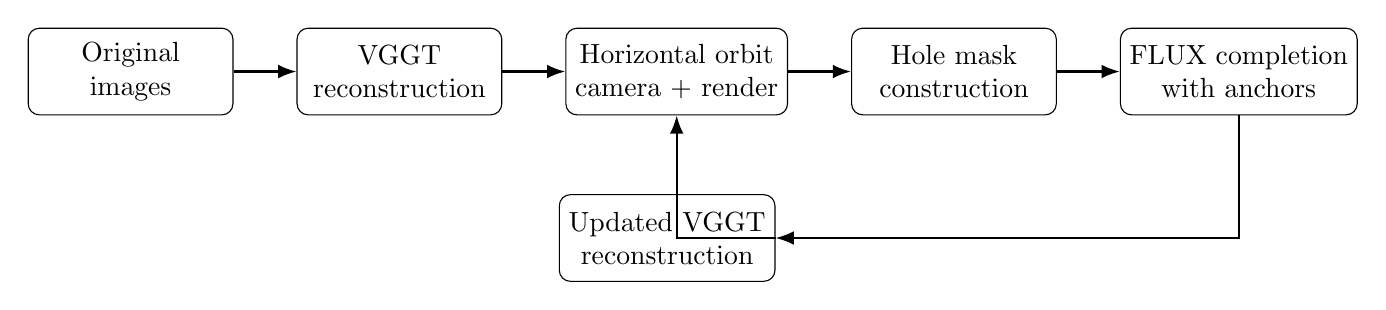
\begin{tikzpicture}[
    node distance=1.0cm and 0.8cm,
    box/.style={draw, rounded corners, align=center, minimum width=2.6cm, minimum height=1.1cm},
    arrow/.style={-Latex, thick}
]
\node[box] (input) {Original\\images};
\node[box, right=of input] (vggt1) {VGGT\\reconstruction};
\node[box, right=of vggt1] (render) {Horizontal orbit\\camera + render};
\node[box, right=of render] (mask) {Hole mask\\construction};
\node[box, right=of mask] (flux) {FLUX completion\\with anchors};
\node[box, below=of vggt1, xshift=3.4cm] (vggt2) {Updated VGGT\\reconstruction};
\draw[arrow] (input) -- (vggt1);
\draw[arrow] (vggt1) -- (render);
\draw[arrow] (render) -- (mask);
\draw[arrow] (mask) -- (flux);
\draw[arrow] (flux) |- (vggt2);
\draw[arrow] (vggt2) -| (render);
\end{tikzpicture}
\caption{Overview of the closed-loop pipeline. The iterative version repeats the rendering and completion steps while updating the reconstruction after each accepted generated view.}
\label{fig:pipeline_overview}
\end{figure}

\subsection{Initial Reconstruction}
The process starts from four real images of the same scene. VGGT reconstructs a point cloud from these inputs and reprojects the result from one of the recovered cameras. This first comparison is important because it checks whether the geometry model already captures the dominant scene structure before any generation is introduced.

\begin{figure}[H]
\centering
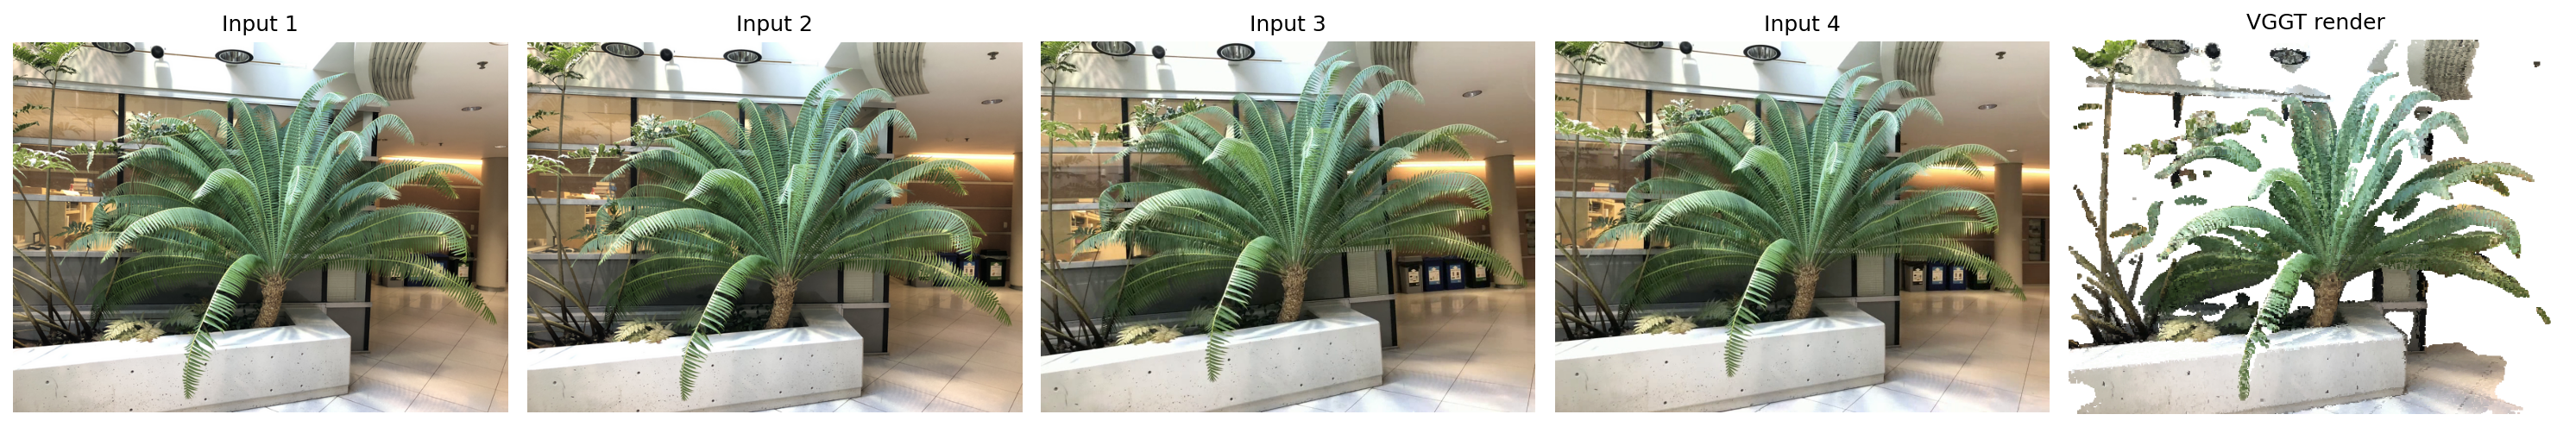
\includegraphics[width=\textwidth]{figures/pipeline_inputs_and_reprojection.png}
\caption{Four original input images and a render of the initial VGGT reconstruction from one recovered camera. The rerender captures coarse scene layout, but it is already sparse and visually close to a flattened point-splat representation rather than a strong 3D reconstruction.}
\label{fig:pipeline_inputs}
\end{figure}

\subsection{Target Camera and Sparse Novel Render}
The iterative version does not move the camera arbitrarily in 3D. It estimates a horizontal orbit around the reconstructed scene, keeps camera height approximately fixed, and selects a target angle inside the largest uncovered angular gap. This produces a sparse target render that points toward unseen regions.

\begin{figure}[H]
\centering
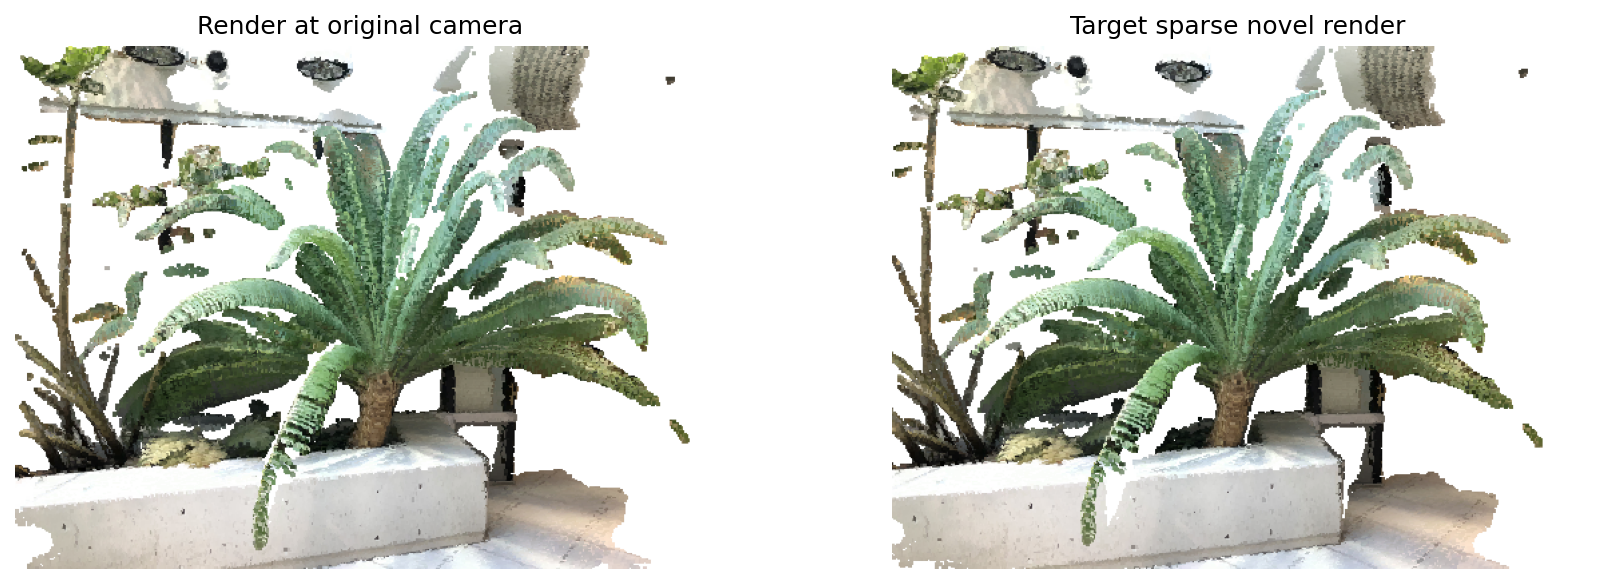
\includegraphics[width=0.82\textwidth]{figures/pipeline_camera_move.png}
\caption{From a render at an existing camera to the target sparse novel render. The horizontal orbit planner improved viewpoint spread compared with the earlier free-plane orbit heuristic.}
\label{fig:pipeline_camera_move}
\end{figure}

\subsection{Hole Detection}
Because the point cloud is incomplete, the target render contains many empty pixels. These holes are identified with a binary mask derived from the render-validity map. The mask is then lightly regularized so that the generator sees coherent missing regions rather than isolated pixels.

\begin{figure}[H]
\centering
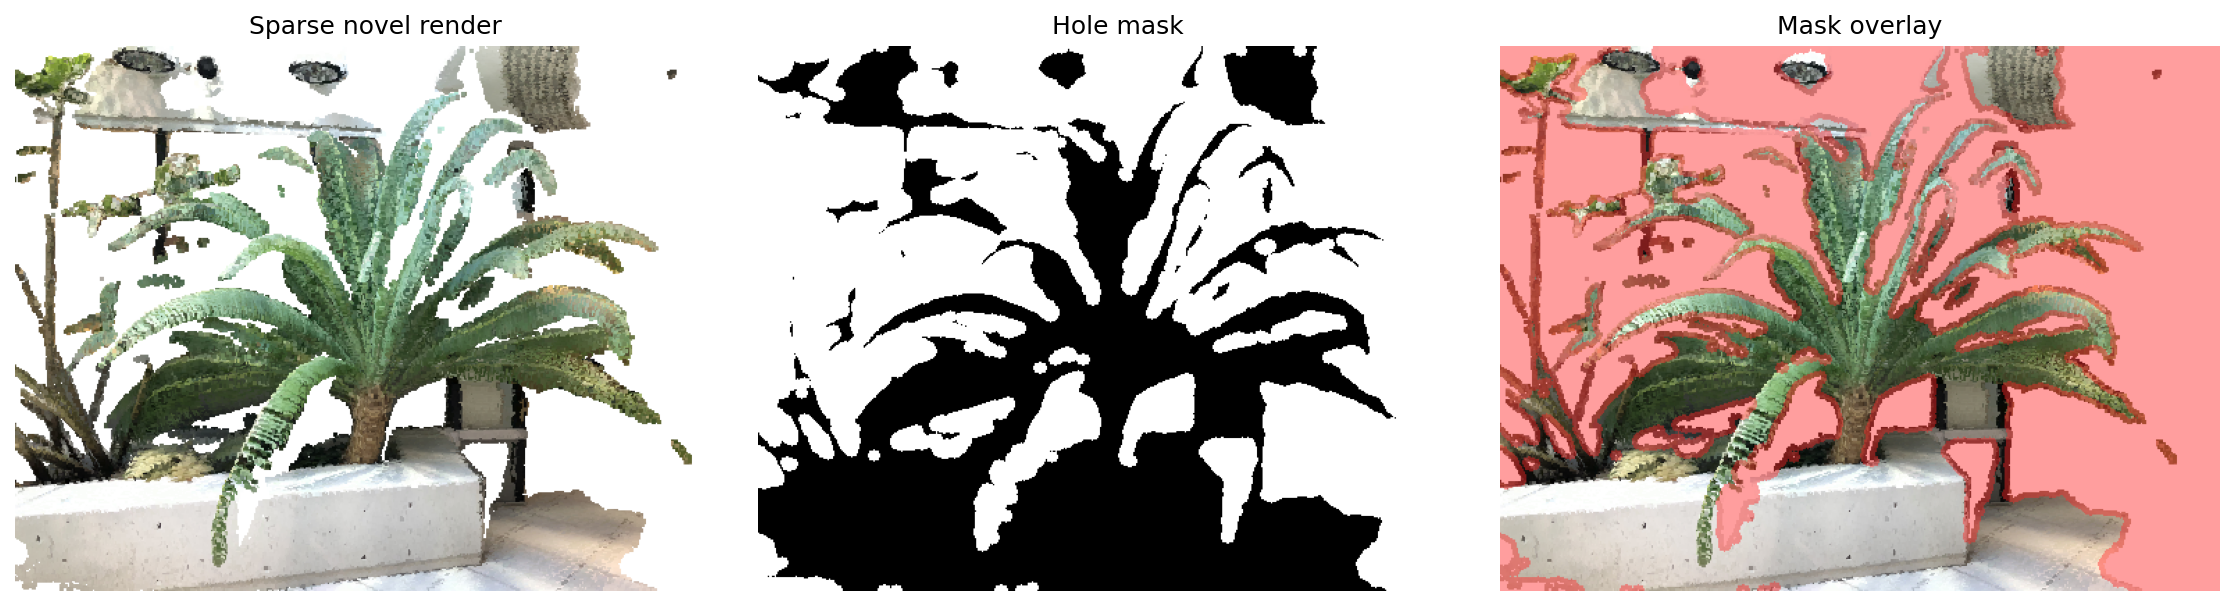
\includegraphics[width=\textwidth]{figures/pipeline_masking.png}
\caption{Sparse novel render, binary hole mask, and mask overlay. The mask marks regions that are not explained by projected geometry and therefore need image completion.}
\label{fig:pipeline_masking}
\end{figure}

\subsection{Novel-View Completion}
The masked target view is passed to FLUX.2-klein together with an anchor sheet built from the original scene images. In this setup, FLUX acts as a reference-guided completion model. Its role is to propose a visually plausible continuation of the sparse target render while staying close to the observed environment.

\begin{figure}[H]
\centering
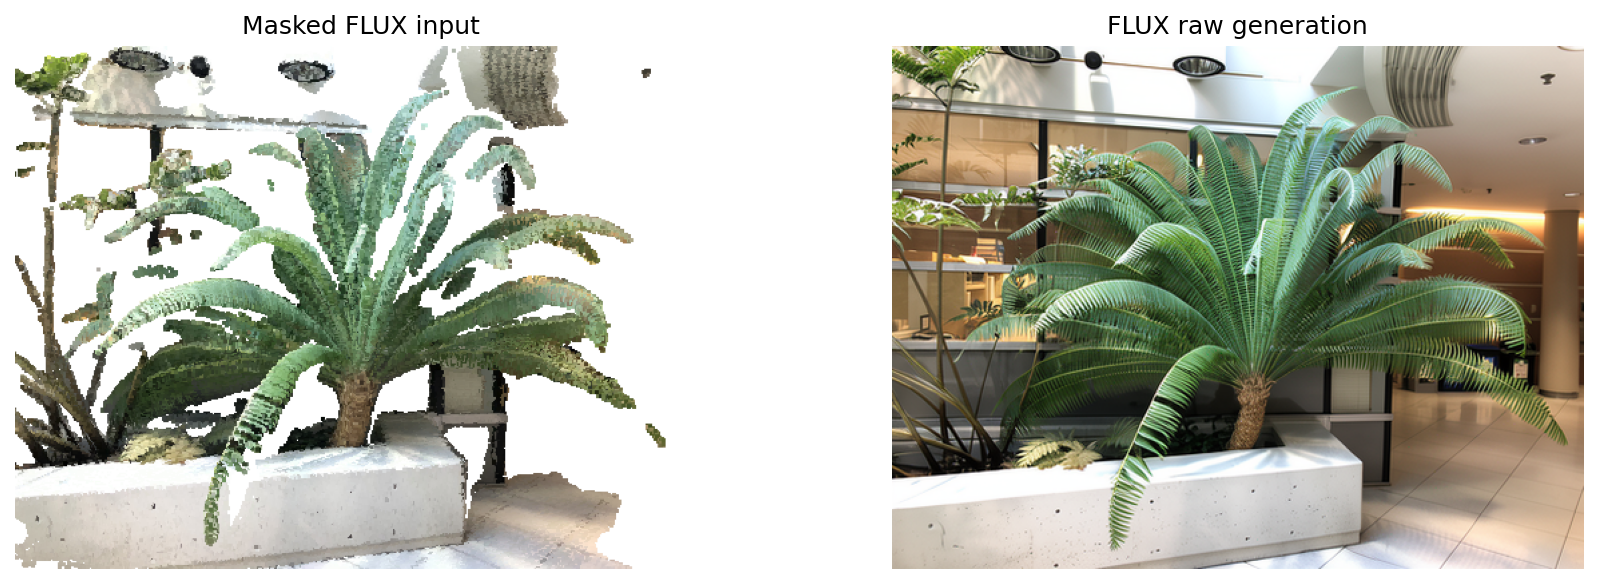
\includegraphics[width=0.82\textwidth]{figures/pipeline_flux_completion.png}
\caption{Masked target image passed to FLUX and the resulting completed view. The generated image is used as the new synthetic observation in the next reconstruction step.}
\label{fig:pipeline_flux}
\end{figure}

\subsection{Reconstruction Update and Validation}
The generated image is appended to the input set and VGGT is run again. The updated point cloud is then compared with the original reconstruction, and the scene is rerendered from the same target pose used for generation. This closes the loop between geometry and image synthesis.

\begin{figure}[H]
\centering
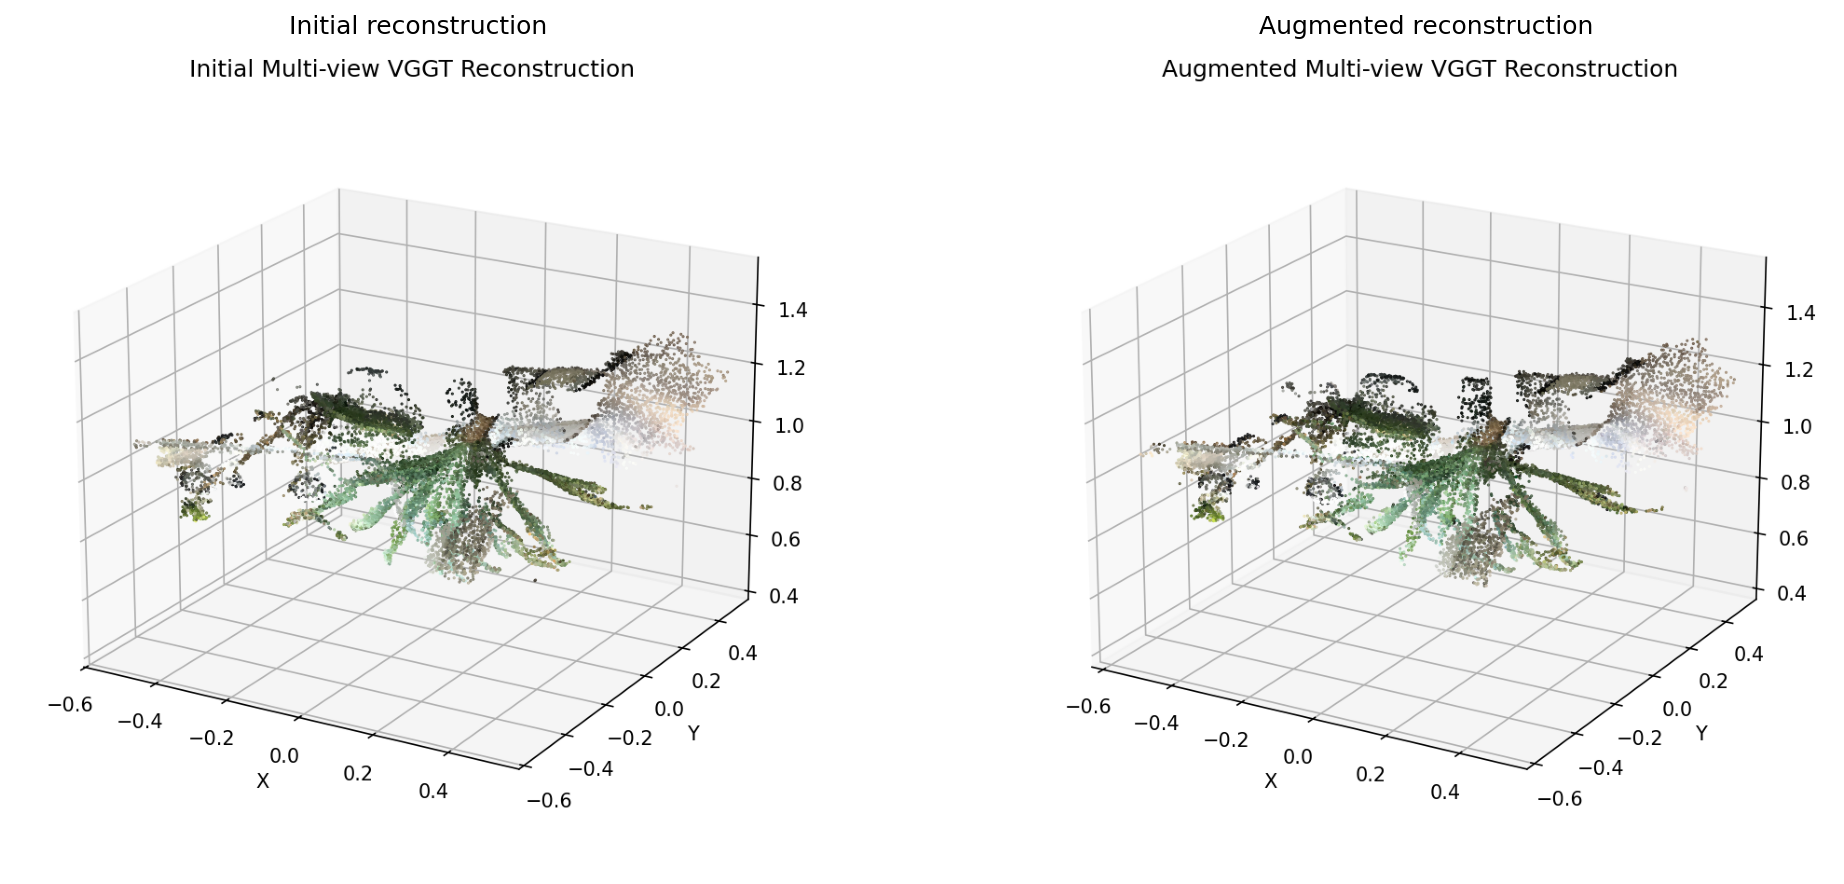
\includegraphics[width=0.82\textwidth]{figures/pipeline_reconstruction_comparison.png}
\caption{Initial reconstruction versus reconstruction after adding the generated novel view. The additional image can improve camera coverage, but the reconstructed geometry remains noisy and only weakly volumetric.}
\label{fig:pipeline_reconstruction}
\end{figure}

\begin{figure}[H]
\centering
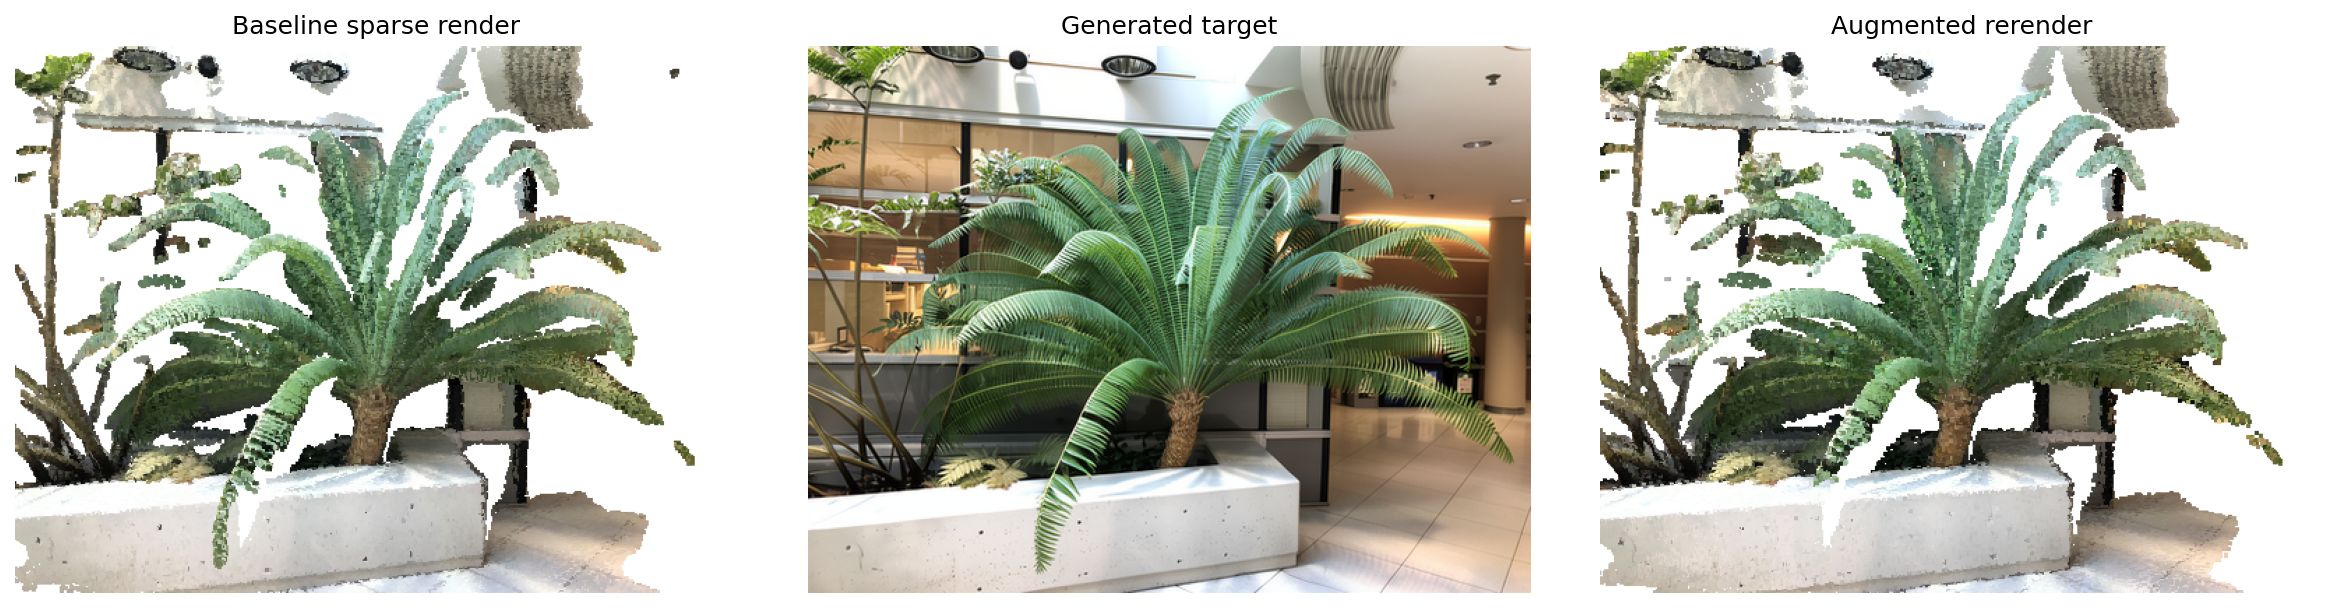
\includegraphics[width=\textwidth]{figures/pipeline_same_pose_rerender.png}
\caption{Baseline sparse render, generated target image, and rerender from the updated reconstruction at the same target pose. This is the single-step bridge between the one-shot experiment and the iterative closed loop.}
\label{fig:pipeline_same_pose}
\end{figure}

\section{Results}
\subsection{Single-Step Bridge}
Before evaluating the closed loop, it is useful to look at the first augmentation step in isolation. Relative to the generated target image, the rerender after reconstruction improves slightly over the sparse baseline in PSNR (\num{7.98} to \num{8.26}) and SSIM (\num{0.224} to \num{0.231}), but becomes slightly worse in LPIPS (\num{0.694} to \num{0.707}). This is not a clearly positive result. The numbers indicate that the rerender gets marginally closer in average pixel intensity and coarse local structure, while becoming less aligned in perceptual feature space. In practice, this usually means that the reconstruction is absorbing broad color and layout cues without faithfully reproducing scene details.

Pose analysis tells a more nuanced story. In the one-step setting, the recovered synthetic camera is close to the intended target in rotation (\num{3.20} degrees), but weak in translation magnitude, with a normalized translation error of \num{1.41}. The generated view also remains closer to one of the original views than desired, which motivates a stronger evaluation over multiple iterations.

\subsection{Iterative Coverage and Pose Fidelity}
The main experiment starts from four real images and adds four generated views, for a total of eight images. Figure~\ref{fig:results_gap} shows the largest unseen angular gap over the loop. Coverage improves from approximately \SI{353.7}{deg} at the start to \SI{248.3}{deg} after four synthetic iterations. This should be interpreted carefully: the metric measures how the recovered cameras spread around the scene, not how accurate or complete the underlying 3D geometry becomes.

\begin{figure}[H]
\centering
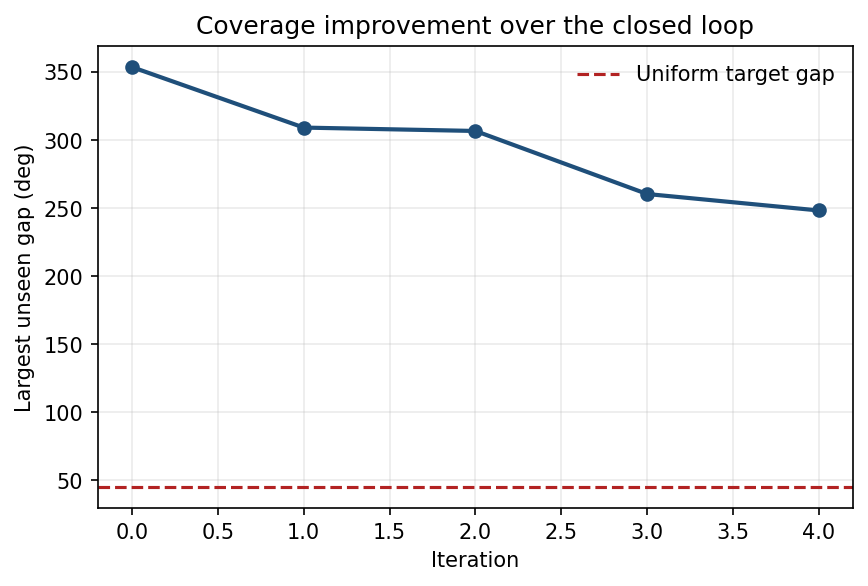
\includegraphics[width=0.75\textwidth]{figures/results_largest_gap_curve.png}
\caption{Largest unseen angular gap over the iterative loop. Lower is better. The horizontal orbit planner reduces unseen coverage substantially over four synthetic updates.}
\label{fig:results_gap}
\end{figure}

However, the gain is not uniform across iterations. Figure~\ref{fig:results_pose} shows the recovered camera error of each generated view. Iterations 1 and 3 are the strongest: their rotation errors are \num{3.36} and \num{5.09} degrees, with normalized translation errors of \num{0.81} and \num{1.68}. By contrast, iterations 2 and 4 drift more strongly, with rotation errors near \num{39} and \num{38} degrees and much larger translation error. The figure is therefore better read as a per-iteration diagnostic than as a smooth convergence curve: two iterations are reasonably pose-consistent, and two fail clearly. This confirms that horizontal orbit planning improved the target selection stage, but generator pose fidelity still varies considerably across iterations.

\begin{figure}[H]
\centering
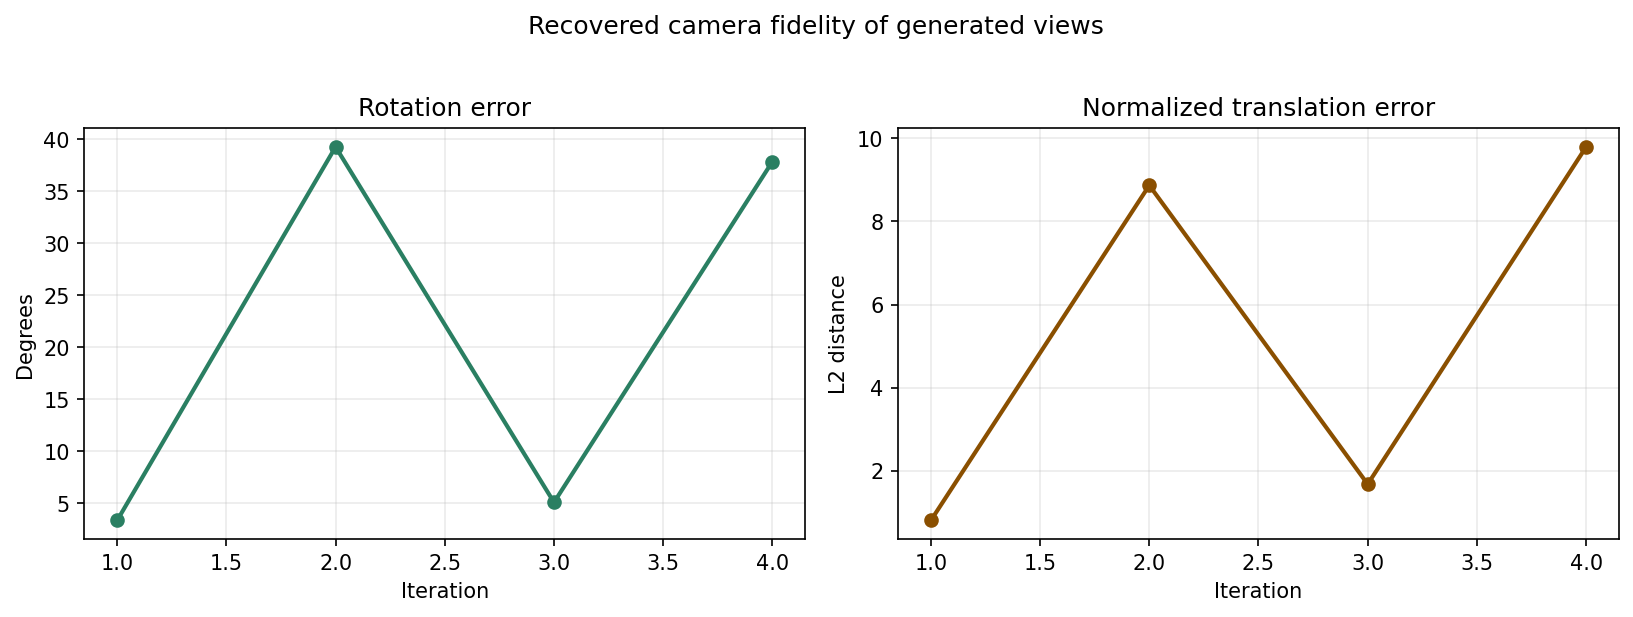
\includegraphics[width=\textwidth]{figures/results_pose_fidelity_curve.png}
\caption{Recovered camera fidelity of generated views across iterations. This plot is not expected to be monotonic; it separates successful and failed synthetic steps. Iterations 1 and 3 remain relatively close to the target pose, while iterations 2 and 4 drift toward already seen viewpoints.}
\label{fig:results_pose}
\end{figure}

\begin{figure}[H]
\centering
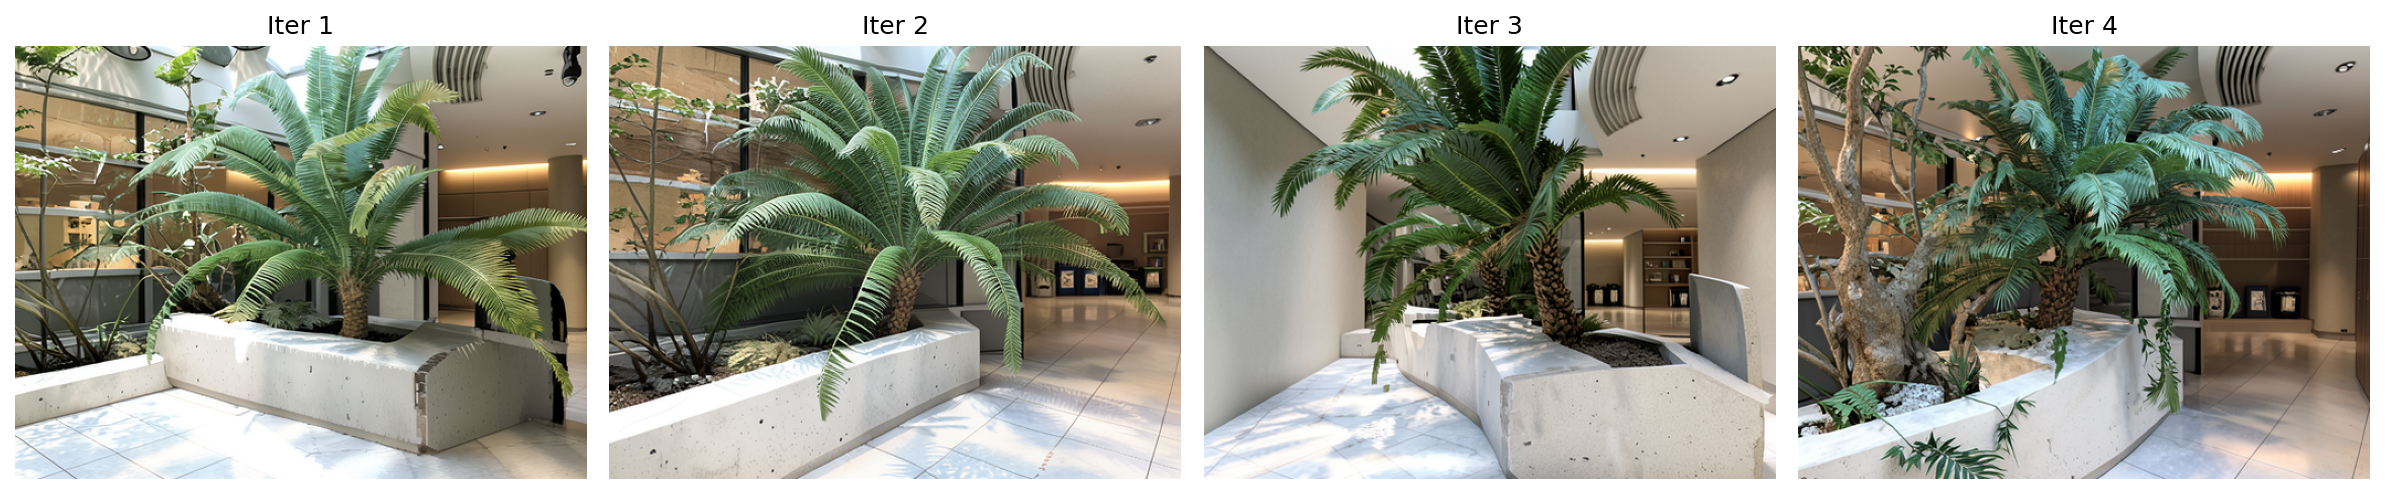
\includegraphics[width=\textwidth]{figures/results_generated_views_strip.png}
\caption{Generated views produced by the four closed-loop iterations. Qualitatively, some steps extend the scene coherently, while others bias back toward existing appearance patterns.}
\label{fig:results_generated}
\end{figure}

\subsection{Preservation of the Original Camera}
To measure whether the loop preserves the observed scene while adding new views, the reconstruction is rerendered from the camera associated with \texttt{image\_01.png} after each iteration. The resulting image is compared with the original photograph using PSNR, SSIM, and LPIPS.

\begin{figure}[H]
\centering
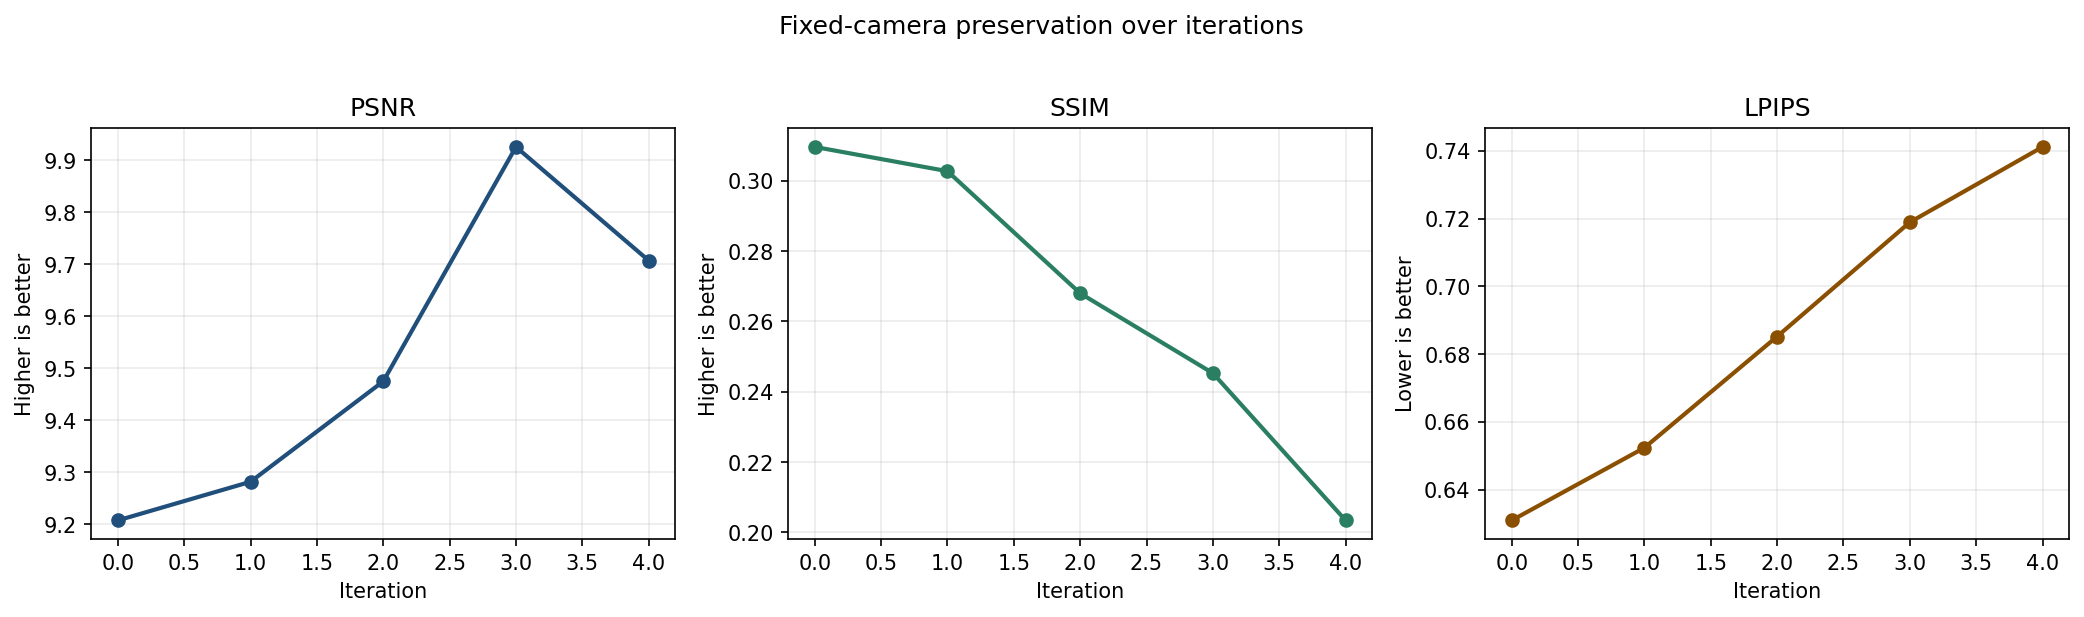
\includegraphics[width=\textwidth]{figures/results_fixed_camera_metrics.png}
\caption{Fixed-camera preservation metrics over the iterative process. PSNR increases modestly, while SSIM and LPIPS degrade, indicating that coarse intensity structure is preserved better than fine perceptual detail.}
\label{fig:results_fixed_camera_metrics}
\end{figure}

The fixed-camera experiment shows a mixed result. PSNR improves from \num{9.21} at the baseline to \num{9.93} after three synthetic iterations, then drops slightly to \num{9.71} at the fourth iteration. In contrast, SSIM declines from \num{0.310} to \num{0.203}, and LPIPS degrades from \num{0.631} to \num{0.741}. Taken together, these trends are not good overall. They indicate that the loop preserves broad brightness and color statistics a little better over time, but it loses structural correspondence and perceptual similarity to the original image.

\begin{figure}[H]
\centering
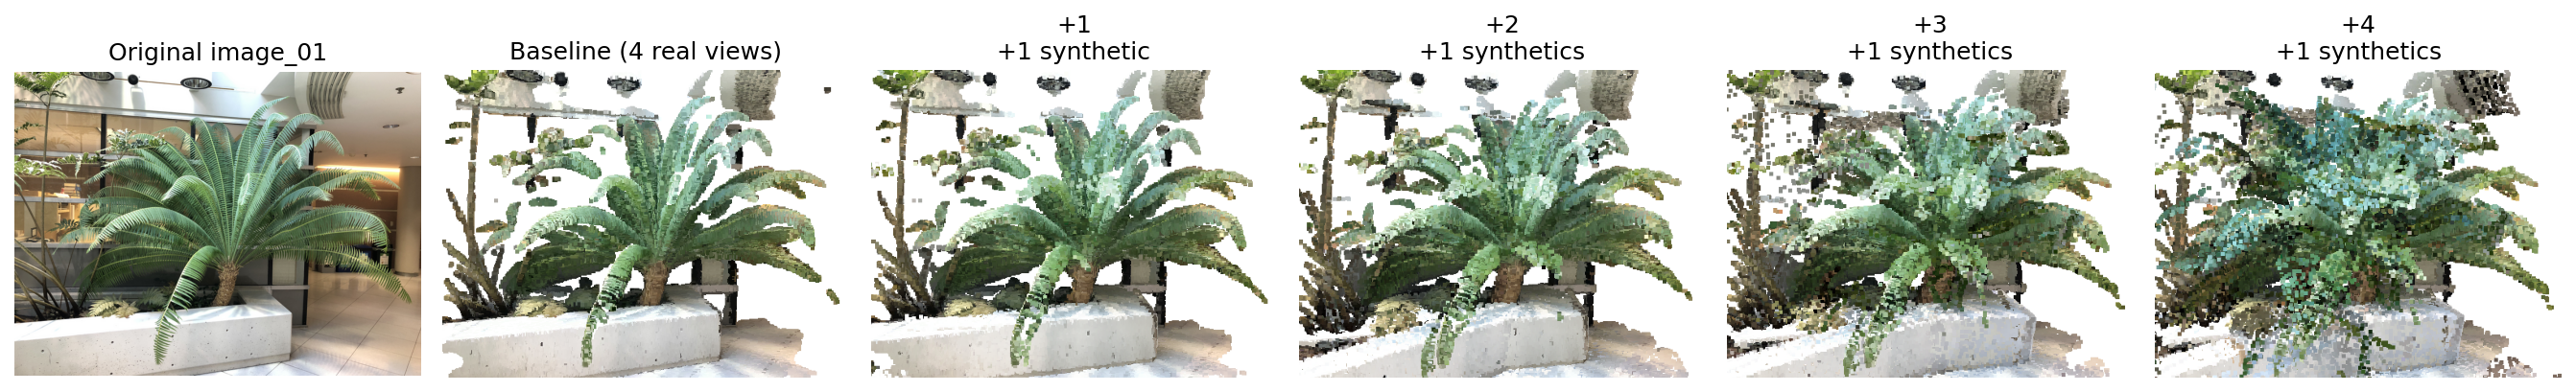
\includegraphics[width=\textwidth]{figures/results_fixed_camera_rerender_strip.png}
\caption{Rerenders from the original camera associated with \texttt{image\_01.png}. The baseline reconstruction is followed by the reconstructions obtained after one to four synthetic additions.}
\label{fig:results_fixed_camera_strip}
\end{figure}

\subsection{Final Reconstruction}
The final reconstruction after four synthetic updates is shown in Figure~\ref{fig:results_final_point_cloud}. The visualization should be read conservatively. The point cloud is still sparse, noisy, and concentrated in a relatively narrow depth range, so it does not yet resemble a high-quality 3D model of the palm tree. The main positive result is improved camera coverage around the object, not a strong final reconstruction. The quantitative results make the same point: visual completion and geometric faithfulness are not equivalent, and some generated views do not remain tightly aligned with the intended target pose.

\begin{figure}[H]
\centering
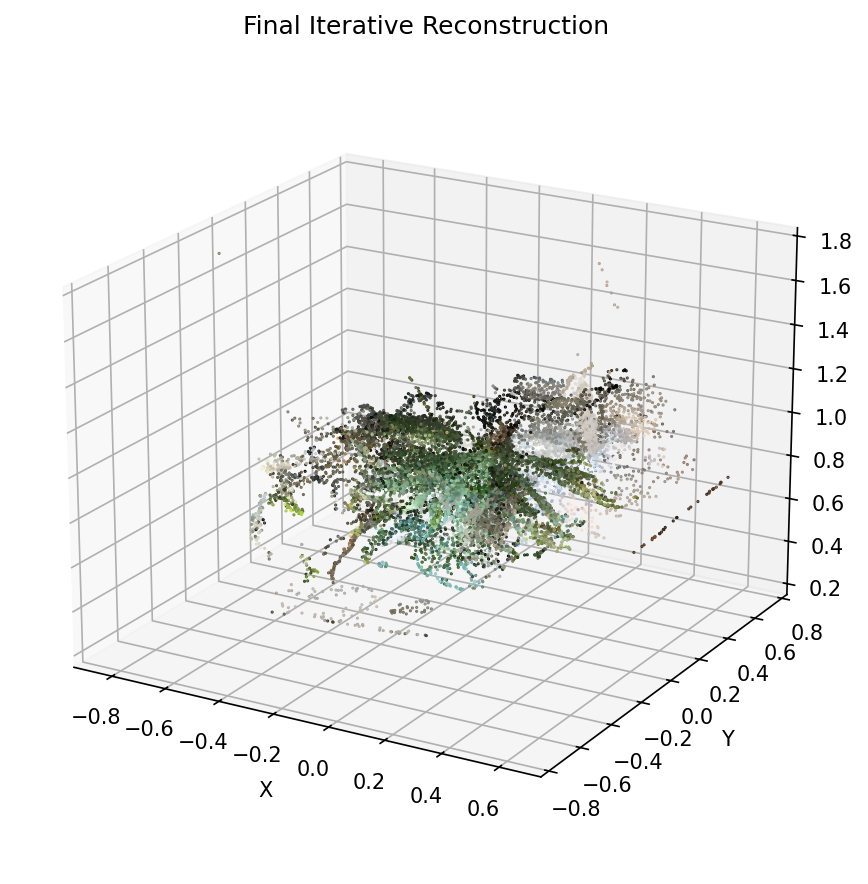
\includegraphics[width=0.72\textwidth]{figures/results_final_point_cloud.png}
\caption{Final point-cloud visualization after four synthetic iterations. The reconstruction spans more viewpoints than the baseline, but it remains a weak and partially flattened point cloud rather than a clean 3D model.}
\label{fig:results_final_point_cloud}
\end{figure}

\section{Conclusion and Future Work}
This project demonstrates that a simple closed-loop combination of geometry reconstruction and image generation can improve sparse-view camera coverage in a measurable way. Starting from four real images, the system expands the set to eight views and reduces the largest unseen angular gap from \SI{353.7}{deg} to \SI{248.3}{deg}. The horizontal orbit planner was an important improvement over the earlier orbit heuristic, because it produced more useful target cameras for this scene.

At the same time, the experiments expose the main limitation of the current system: FLUX.2-klein is lightweight and practical, but not sufficiently pose-faithful for stable iterative expansion. Some generated views match the intended orbit well, while others drift back toward already observed viewpoints. This inconsistency also appears in the fixed-camera preservation study, where SSIM and LPIPS deteriorate across iterations even when the camera-distribution metric improves. The resulting reconstructions therefore remain sparse and only weakly 3D.

The hardware budget is another real constraint. A larger run with ten total views exceeded available MPS memory during reconstruction, so the final experiment was limited to eight views. This is a practical limitation rather than a conceptual one. Future work should therefore target three directions: a stronger pose-conditioned completion model, an explicit acceptance or rejection rule based on recovered camera pose, and more capable compute or paid inference access. With a larger model or a higher-quality external service such as Nano Banana, the same loop could likely produce more informative and more stable synthetic views.

\bibliographystyle{plainnat}
\bibliography{references}

\end{document}
